\documentclass{beamer}
\usepackage{mathspec}
\usepackage{xeCJK}
\setCJKmainfont{IPAPMincho}
\setCJKsansfont{IPAGothic}
\setCJKmonofont{IPAGothic}

% You can set fonts for Latin script here
\setmainfont{FreeSerif}
\setsansfont{FreeSans}
\setmonofont{Latin Modern Mono}

\usetheme{DarkConsole}

\setbeamertemplate{theorems}[normal font]

\title{Demo}
\subtitle{}
\author{Sofía Almeida Bruno\\\qquad\quad Fernando de la Hoz Moreno}
\date{}

%%%%%%%%%%%%%%%%%%%%%%%%%%%%%%%%%%%%%%%%%%%%%%%%%%%%%%%%%%%%%%%%%%%%%%%%%%%
%%%						COMIENZO DEL DOCUMENTO							%%%
%%%%%%%%%%%%%%%%%%%%%%%%%%%%%%%%%%%%%%%%%%%%%%%%%%%%%%%%%%%%%%%%%%%%%%%%%%%
\begin{document}

\begin{frame}
  \maketitle
\end{frame}

\begin{frame}
	En esta demostración utilizamos dos máquinas virtuales: una de Kali Linux y otra de WindowsXP. Ambas deben estar en la misma red.\\
	
	Para comprobar que las máquinas se ven enviaremos un ping entre ellas.\\
	
	Desde Kali Linux, intentaremos atacar la máquina WindowsXP combinando Nmap, Nessus y metaesploit.
\end{frame}

\begin{frame}

Utilizamos Nmap para ver qué puertos tiene abiertos y con qué servicios:

\begin{figure}[h]
\centering
		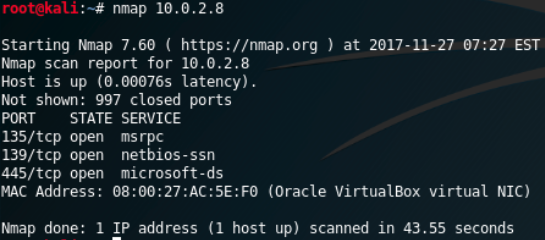
\includegraphics[scale=0.5]{./img/Demo/Nmap1}
\end{figure}

\end{frame}

\begin{frame}

Iniciamos Nessus, un demonio que actúa como servidor.

\begin{figure}[h]
\centering
		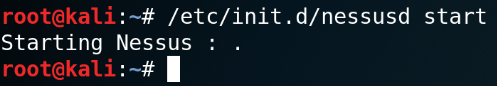
\includegraphics[scale=0.5]{./img/Demo/Nessus1}
\end{figure}
\end{frame}

\begin{frame}

Nos conectamos a un cliente gráfico de Nessus a través del navegador web y escaneamos el equipo que deseamos atacar.

\begin{figure}[h]
\centering
		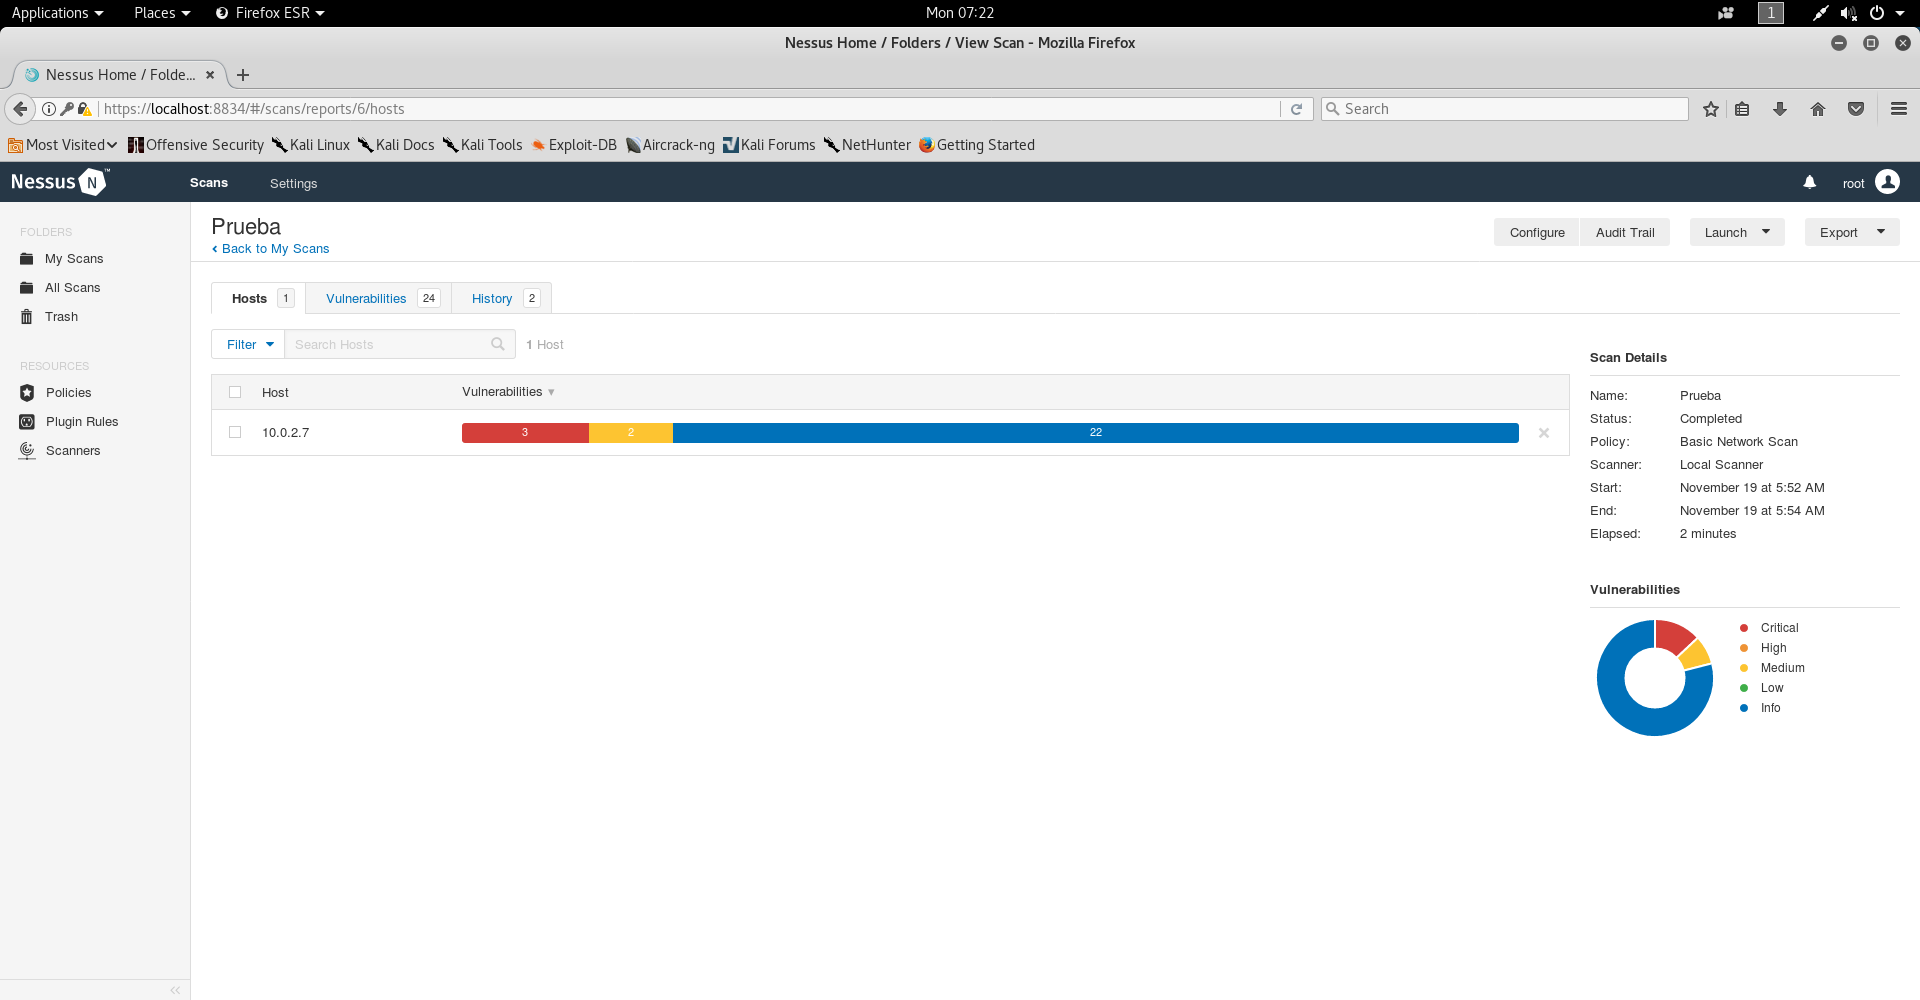
\includegraphics[scale=0.25]{./img/Demo/Nessus2}
\end{figure}
\end{frame}

\begin{frame}
\begin{figure}[h]
\centering
		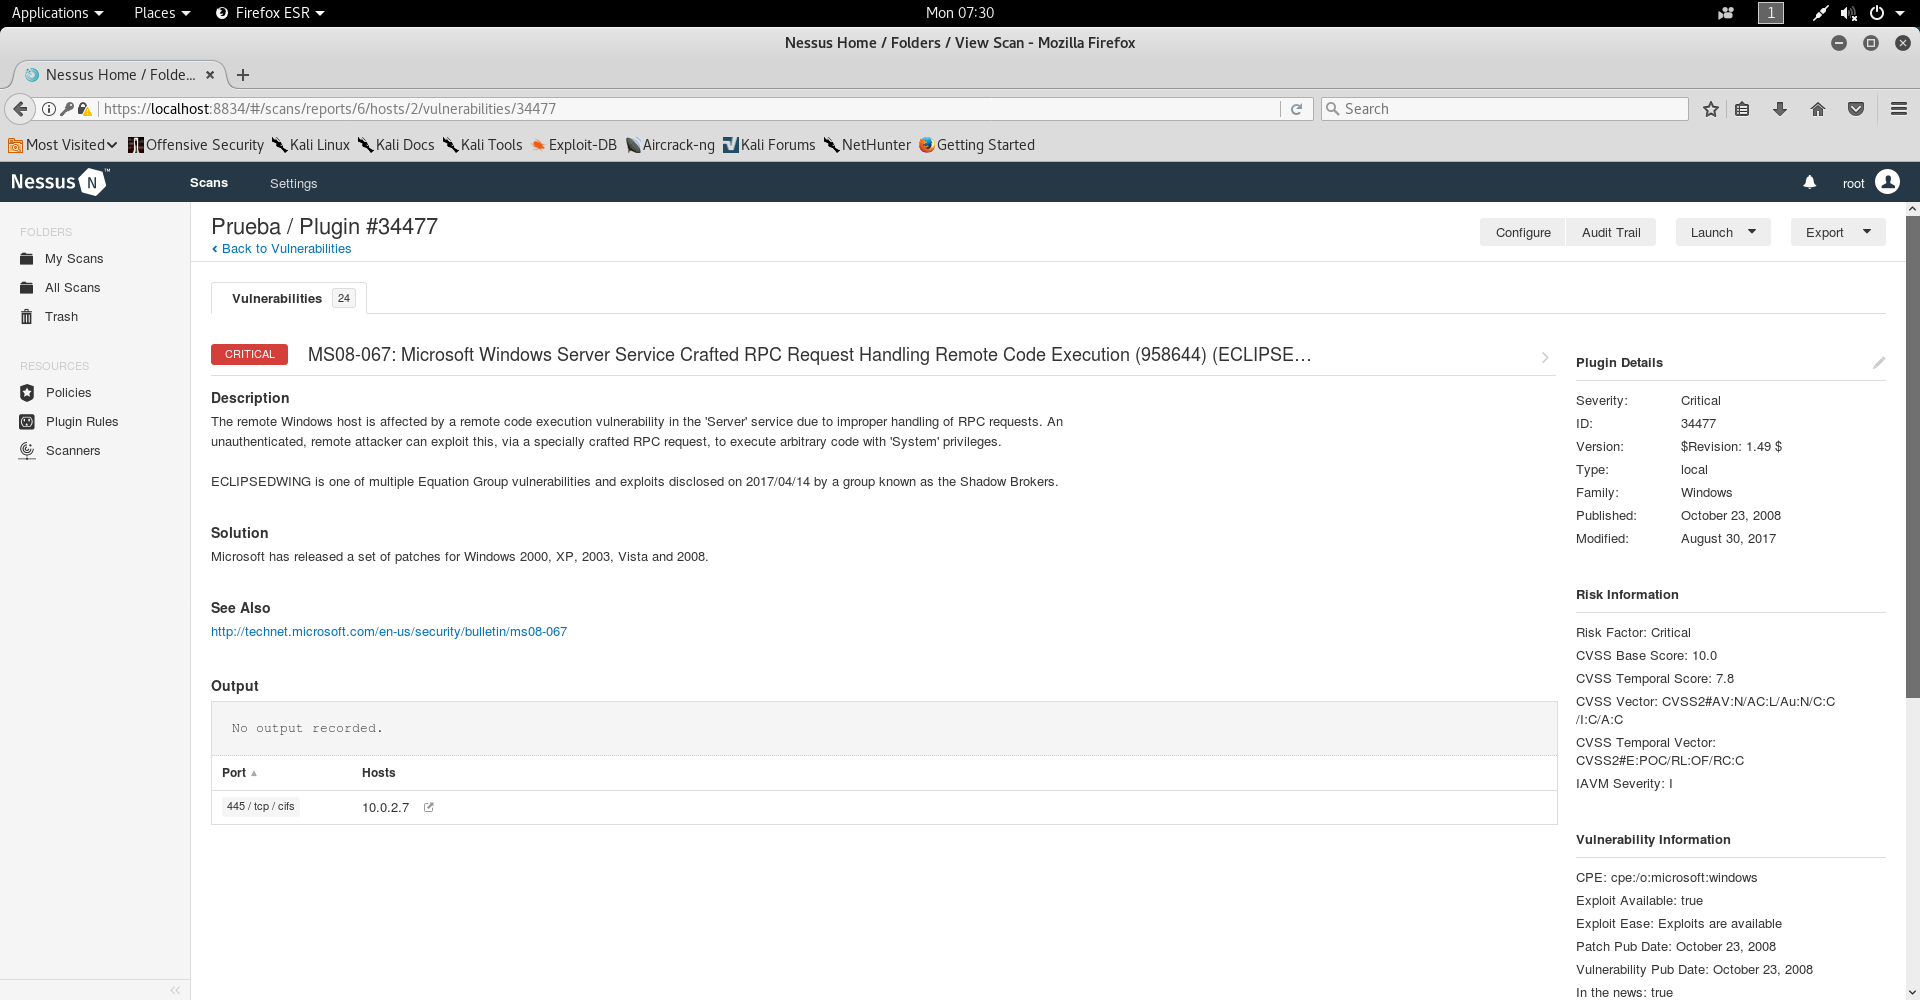
\includegraphics[scale=0.25]{./img/Demo/Nessus3}
\end{figure}
\end{frame}

\begin{frame}
	Iniciamos Metaesploit
	\begin{figure}[h]
\centering
		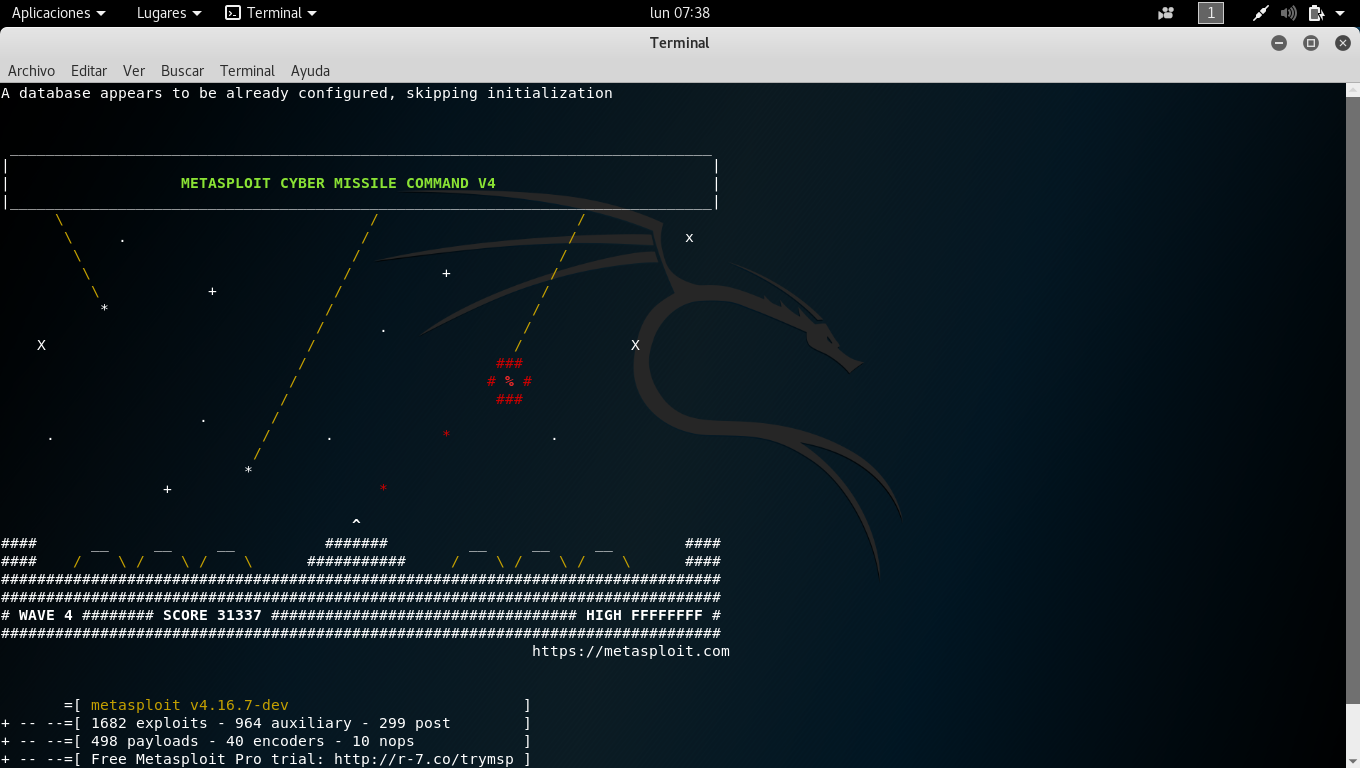
\includegraphics[scale=0.3]{./img/Demo/Metasploit1}
\end{figure}
\end{frame}

\begin{frame}
	\begin{figure}[h]
\centering
		\includegraphics[scale=0.3]{./img/Demo/Metasploit2}
\end{figure}
\end{frame}

\begin{frame}
	\begin{figure}[h]
\centering
		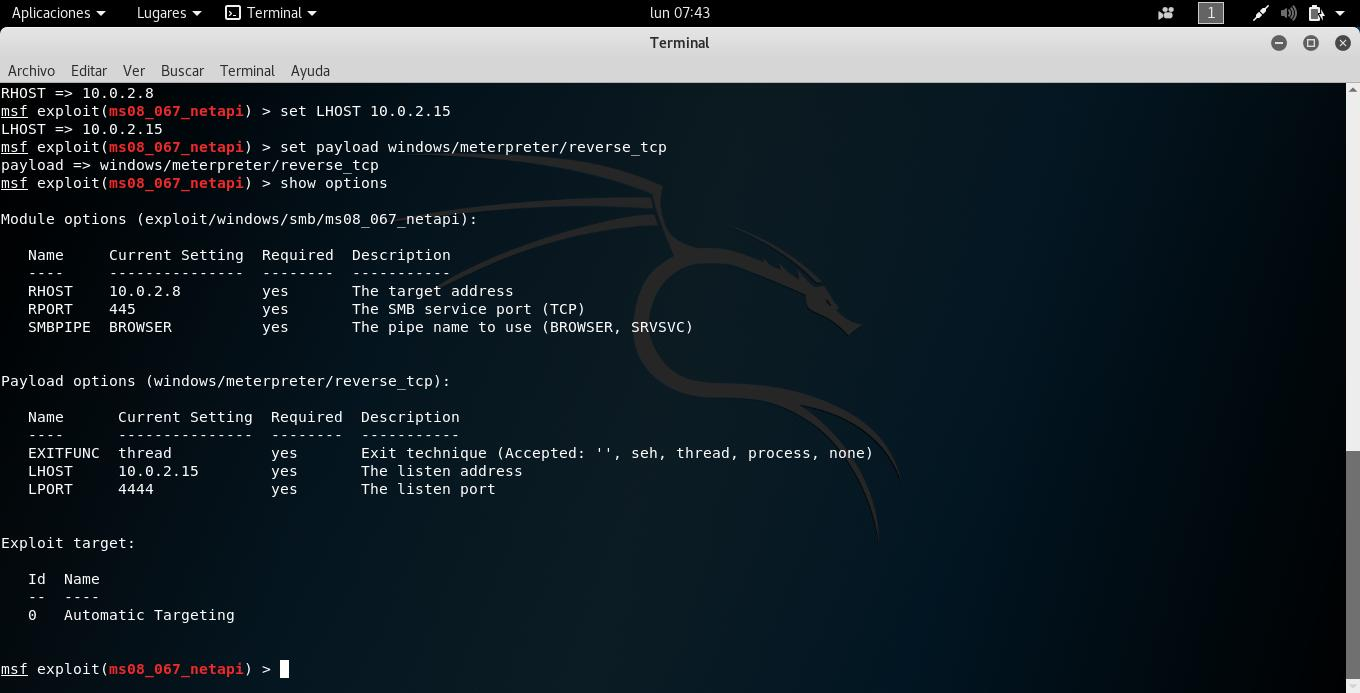
\includegraphics[scale=0.3]{./img/Demo/Metasploit3}
\end{figure}
\end{frame}

\begin{frame}
	\begin{figure}[h]
\centering
		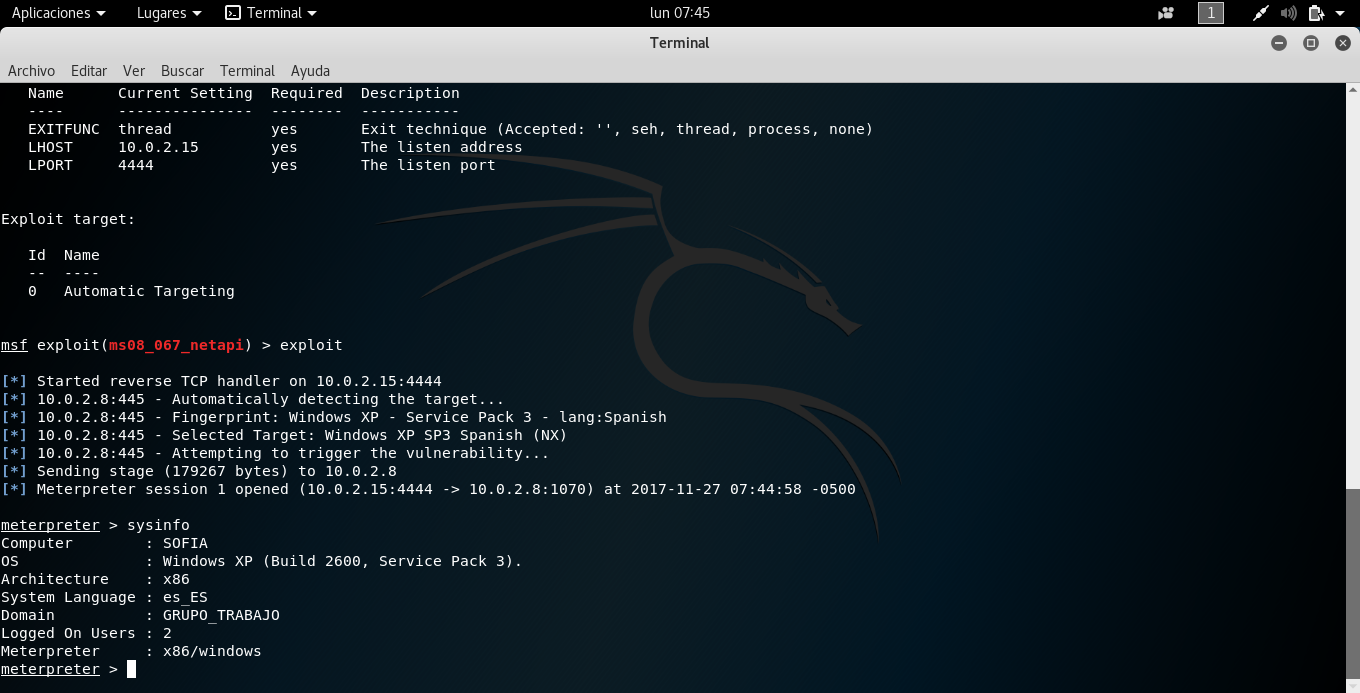
\includegraphics[scale=0.3]{./img/Demo/Metasploit4}
\end{figure}
\end{frame}

\end{document}
